% \subsection{Strategy}

% ===============================================================================================================================
\begin{frame}{Gamma-ray bursts}
\centering
\begin{tikzpicture}
  % Alert
  \node at (0,3) [above] {Alerts};
  \fill [color=tuorange, fill opacity=0.2] (-1.2,3) rectangle (1.2, -3);
  % \draw (0,1.5) circle [minimum size=1] node [align=left] {SWIFT,\\Fermi-GBM,\\SVOM};
  \node [draw,circle, minimum size=1, align=left] (A1) at (0,1.5) {SWIFT,\\Fermi-GBM,\\SVOM};
  % \draw (0,-1.5) circle [minimum size=1] node [align=left] {Fermi-LAT,\\DAMPE,\\HAWC, etc.};
  \node [draw,circle, minimum size=1, align=left] (A2) at (0,-1.5) {Fermi-LAT,\\DAMPE,\\HAWC, etc.};

  % CTA
  \uncover<2->{
  \node at (6,3) [above] {Cherenkov Telescope Array};
  \fill [color=tugreen, fill opacity=0.3] (1.8,3) rectangle (10.2, -3);
  % \draw (3,0) circle [minimum size=1] node [align=left] {dark time?};
  \node [draw,circle, minimum size=1] (B) at (3,0) {dark time?};
  \draw[gray,->, >=stealth, to path={-| (\tikztotarget)}]
  (A2) edge (B);
  \draw[->, >=stealth, to path={-| (\tikztotarget)}]
  (A1) edge (B);

  \node at (2.2,-1.5) [below, color=gray] {rarely};
  }

  \uncover<3->{
  % \draw (6,1.5) circle [minimum size=1] node [align=left] {late-time\\follow-up};
  \node [draw,circle, minimum size=1, align=left] (C1) at (6,1.5) {late-time\\follow-up};
  % \draw (6,-1.5) circle [minimum size=1] node [align=left] {full-array\\follow-up};
  \node [draw,circle, minimum size=1, align=left] (C2) at (6,-1.5) {full-array\\follow-up};
  \draw[->, >=stealth, to path={-- (\tikztotarget)}]
  (B) edge (C1) (B) edge (C2);

  \node at (4.1,1.2) [below] {no};
  \node at (4.1,-1.2) [above] {yes};
  }

  \uncover<4->{
  % \draw (9,-1.5) circle [minimum size=1] node [align=center] {extend\\observation\\time};
  \node [draw,circle, minimum size=1, align=center] (D) at (9,-1.5) {extend\\observation\\time};
  \draw[->, >=stealth, to path={-| (\tikztotarget)}]
  (C1) edge (D);
  \draw[->, >=stealth, to path={-- (\tikztotarget)}]
  (C2) edge (D);

  \node at (7.9,1.5) [above] {detection};
  \node at (7.4,-1.5) [below] {detection};
  }

  \uncover<5->{
  % \draw (12,-1.5) circle [minimum size=1] node [align=center] {MWL\\follow-up};
  \node [draw,circle, minimum size=1, align=center] (E) at (12,-1.5) {MWL\\follow-up};
  \draw[->, >=stealth, to path={-- (\tikztotarget)}]
  (D) edge (E);
  }

\end{tikzpicture}
\end{frame}

% ===============================================================================================================================
\begin{frame}{Galactic Transients}
  \centering
  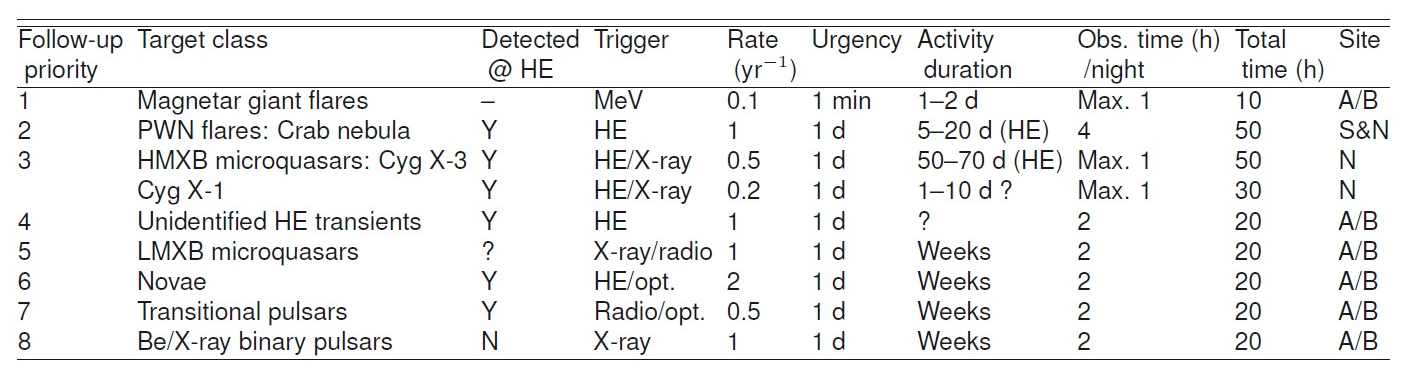
\includegraphics[width=0.8\textwidth]{graphics/galactic_table_full.png}
  \begin{itemize}
    \item Targets prioritized based on their rarity or duration of activity
    \item Simultaneous MWL follow-up for maximized scientific output
  \end{itemize}
\end{frame}

% ===============================================================================================================================
\begin{frame}{X-ray, optical, and radio transients}
\begin{itemize}
  \item Existing alert systems for current IACTs can be used by CTA
  \item Follow-up strategies prove to be challenging
  \begin{itemize}
    \item [\to] Numerous uncertainties concerning performance of each facility, latency for recieving different types of alerts
  \end{itemize}
  \item Outlining possible strategies for "slower" Galactic transients depending on:
  \begin{itemize}
    \item [\to] Expectations of optical transient facilities to discover large quantities of novae
    \item [\to] Search for VHE gamma rays from known objects by current IACTs
  \end{itemize}
  \item Base filtering criteria on optical magnitude, nova type, properties of HE gamma rays, etc.
\end{itemize}
\begin{center}
  \textcolor{tugreen}{$\Longrightarrow$} Development of optimal methodology is critical
\end{center}

\end{frame}

% ===============================================================================================================================
\begin{frame}{HE neutrino transients}
  \centering
  \begin{tikzpicture}[scale=0.750, every node/.style={scale=0.8}]
    % Alert
    \node at (3,3) [above] {Alerts};
    \fill [color=tublue, fill opacity=0.2] (-1.2,3) rectangle (7.5, -3);
    \node [draw,circle, minimum size=1] (A) at (0,0) {IceCube};

    \uncover<2->{
    % \fill [color=tugreen, fill opacity=0.3] (1.8,3) rectangle (10.2, -3);
    \node [draw,circle, minimum size=1, align=center] (B1) at (3,2) {Upgoing\\multiplets};
    \node [draw,circle, minimum size=1, align=center] (B2) at (3,0) {Extremely\\HE events};
    \node [draw,circle, minimum size=1, align=center] (B3) at (3,-2) {HE\\starting\\events};
    \draw[->, >=stealth, to path={-- (\tikztotarget)}]
    (A) edge (B1) (A) edge (B2) (A) edge (B3);
    % \node at (2.2,-1.5) [below, color=gray] {rarely};
    }

    \uncover<3->{
    \node [draw,circle, minimum size=1, align=center, scale=0.85] (C2) at (6,0) {real-time,\\online system};
    \draw[->, >=stealth, to path={-- (\tikztotarget)}]
    (B2) edge (C2);
    }

    \uncover<4->{
    \node [draw,circle, minimum size=1, align=center, scale=0.85] (C3) at (6,-2) {alternative\\real-time,\\online system};
    \draw[->, >=stealth, to path={-- (\tikztotarget)}]
    (B3) edge (C3);
    }

    \uncover<5->{
    \node at (9,3) [above] {CTA};
    \fill [color=tugreen, fill opacity=0.2] (7.8,3) rectangle (10.2, -3);
    \node [draw,circle, minimum size=1] (D) at (9,0) {CTA};
    \coordinate (k) at (7.5,0);
    \draw[to path={-| (\tikztotarget)}]
    (B1) to (k) (C3) edge (k);
    \draw[to path={-- (\tikztotarget)}]
    (C2) to (k);
    \draw[->, >=stealth, to path={-- (\tikztotarget)}]
    (k) to (D);

    \node [draw,dashed,circle, minimum size=1,scale=0.3] (nD) at (9.2,-2.5) {
      \begin{tikzpicture}[anchor=center]
        \node [draw,circle, minimum size=1] (nB) at (6,0) {dark time?};

        \node [draw,circle, minimum size=1, align=left] (nC1) at (9,1.5) {late-time\\follow-up};
        \node [draw,circle, minimum size=1, align=left] (nC2) at (9,-1.5) {full-array\\follow-up};
        \draw[->, >=stealth, to path={-- (\tikztotarget)}]
        (nB) edge (nC1) (nB) edge (nC2);

        \node at (7.1,1.2) [below] {no};
        \node at (7.1,-1.2) [above] {yes};

        % \draw (9,-1.5) circle [minimum size=1] node [align=center] {extend\\observation\\time};
        \node [draw,circle, minimum size=1, align=center] (nD) at (12,-1.5) {extend\\observation\\time};
        \draw[->, >=stealth, to path={-| (\tikztotarget)}]
        (nC1) edge (nD);
        \draw[->, >=stealth, to path={-- (\tikztotarget)}]
        (nC2) edge (nD);

        \node at (10.9,1.5) [above] {detection};
        \node at (10.4,-1.5) [below] {\small detection};
      \end{tikzpicture}
      };
      \draw[dashed, to path={-- (\tikztotarget)}]
      (D) edge (nD);
    }

    \uncover<6->{
    \node [draw,circle, minimum size=1, align=center] (E) at (12,0) {MWL\\follow-up};
    \draw[->, >=stealth, to path={-- (\tikztotarget)}]
    (D) edge (E);
    }
  \end{tikzpicture}
\end{frame}

% ===============================================================================================================================
\begin{frame}{GW transients}
  \centering
  \begin{tikzpicture}%[scale=0.750, every node/.style={scale=0.8}]
    % Alert
    \node at (0,3) [above] {Alerts};
    \fill [color=tuviolet, fill opacity=0.2] (-1.2,3) rectangle (1.2, -3);
    \node [draw,circle, minimum size=1] (A) at (0,0) {LIGO/VIRGO};

    \uncover<2->{
    \node at (4.65,3) [above] {CTA};
    \fill [color=tugreen, fill opacity=0.2] (1.8,3) rectangle (7.5, -3);
    \node [draw,circle, minimum size=1] (B) at (3,0) {CTA};
    \draw[->, >=stealth, to path={-- (\tikztotarget)}]
    (A) edge (B);

    \node [draw,dashed,circle, minimum size=1,scale=0.3] (nB) at (3.2,-2.5) {
      \begin{tikzpicture}[anchor=center]
        \node [draw,circle, minimum size=1] (nB) at (6,0) {dark time?};

        \node [draw,circle, minimum size=1, align=left] (nC1) at (9,1.5) {late-time\\follow-up};
        \node [draw,circle, minimum size=1, align=left] (nC2) at (9,-1.5) {full-array\\follow-up};
        \draw[->, >=stealth, to path={-- (\tikztotarget)}]
        (nB) edge (nC1) (nB) edge (nC2);

        \node at (7.1,1.2) [below] {no};
        \node at (7.1,-1.2) [above] {yes};

        % \draw (9,-1.5) circle [minimum size=1] node [align=center] {extend\\observation\\time};
        \node [draw,circle, minimum size=1, align=center] (nD) at (12,-1.5) {extend\\observation\\time};
        \draw[->, >=stealth, to path={-| (\tikztotarget)}]
        (nC1) edge (nD);
        \draw[->, >=stealth, to path={-- (\tikztotarget)}]
        (nC2) edge (nD);

        \node at (10.9,1.5) [above] {detection};
        \node at (10.4,-1.5) [below] {\small detection};
      \end{tikzpicture}
      };
      \draw[dashed, to path={-- (\tikztotarget)}]
      (B) edge (nB);
    }

    \uncover<3->{
    \node [draw,circle, minimum size=1, align=center] (C) at (6,0) {Tiling or\\divergent pointing};
    \draw[->, >=stealth, to path={-- (\tikztotarget)}]
    (B) edge (C);
    }

    \uncover<4->{
    \node [draw,circle, minimum size=1, align=center] (D) at (9,0) {MWL\\follow-up};
    \draw[->, >=stealth, to path={-- (\tikztotarget)}]
    (C) edge (D);
    }
  \end{tikzpicture}
\end{frame}

% ===============================================================================================================================
\begin{frame}{Serendipitous VHE transients}
  \centering
  \begin{tikzpicture}%[scale=0.750, every node/.style={scale=0.8}]
    % Alert
    \node at (0,3) [above] {Alerts};
    \node at (3,3) [above] {CTA};
    \fill [color=tugreen, fill opacity=0.2] (-1.2,3) rectangle (7.5, -3);
    \node [draw,circle, minimum size=1] (A) at (0,0) {RTA};

    \uncover<2->{
    \node [draw,circle, minimum size=1,align=center] (B) at (3,0) {short-term\\scheduler};
    \draw[->, >=stealth, to path={-- (\tikztotarget)}]
    (A) edge (B);
    \node at (1.2,0) [above] {detection};
    }

    \uncover<3->{
    \node [draw,circle, minimum size=1, align=center] (D) at (9,0) {MWL\\follow-up};
    \draw[->, >=stealth, to path={-- (\tikztotarget)}]
    (B) edge (D);
    }

    \uncover<4->{
    \node [draw,circle, minimum size=1, align=center] (C) at (6,2) {on-site\\data analysis};
    \draw[->, >=stealth, to path={-- (\tikztotarget)}]
    (B) edge (C);
    }
  \end{tikzpicture}
\end{frame}

% ===============================================================================================================================
\begin{frame}{VHE transient survey}
  \begin{itemize}
    \item Conducted via suitable divergent pointing pattern
    \begin{itemize}
      \item [\to] 20 deg FoV for searches of relatively bright transients
    \end{itemize}
    \item Increasing the FoV results in decreased sensitivity and increased energy threshold
    \begin{itemize}
      \item [\to] Compromise is critical
    \end{itemize}  
    \item Targeting regions at high Galactic latitudes are strongly favoured
    \item Using the RTA systems for automatic identification of transients to alert for MWL follow-up
  \end{itemize}
\end{frame}
